\begin{frame}{Effects of Sublimation near Mamers Valles}

\begin{figure}
\centering
\begin{subfigure}{0.48\textwidth}
    \centering
    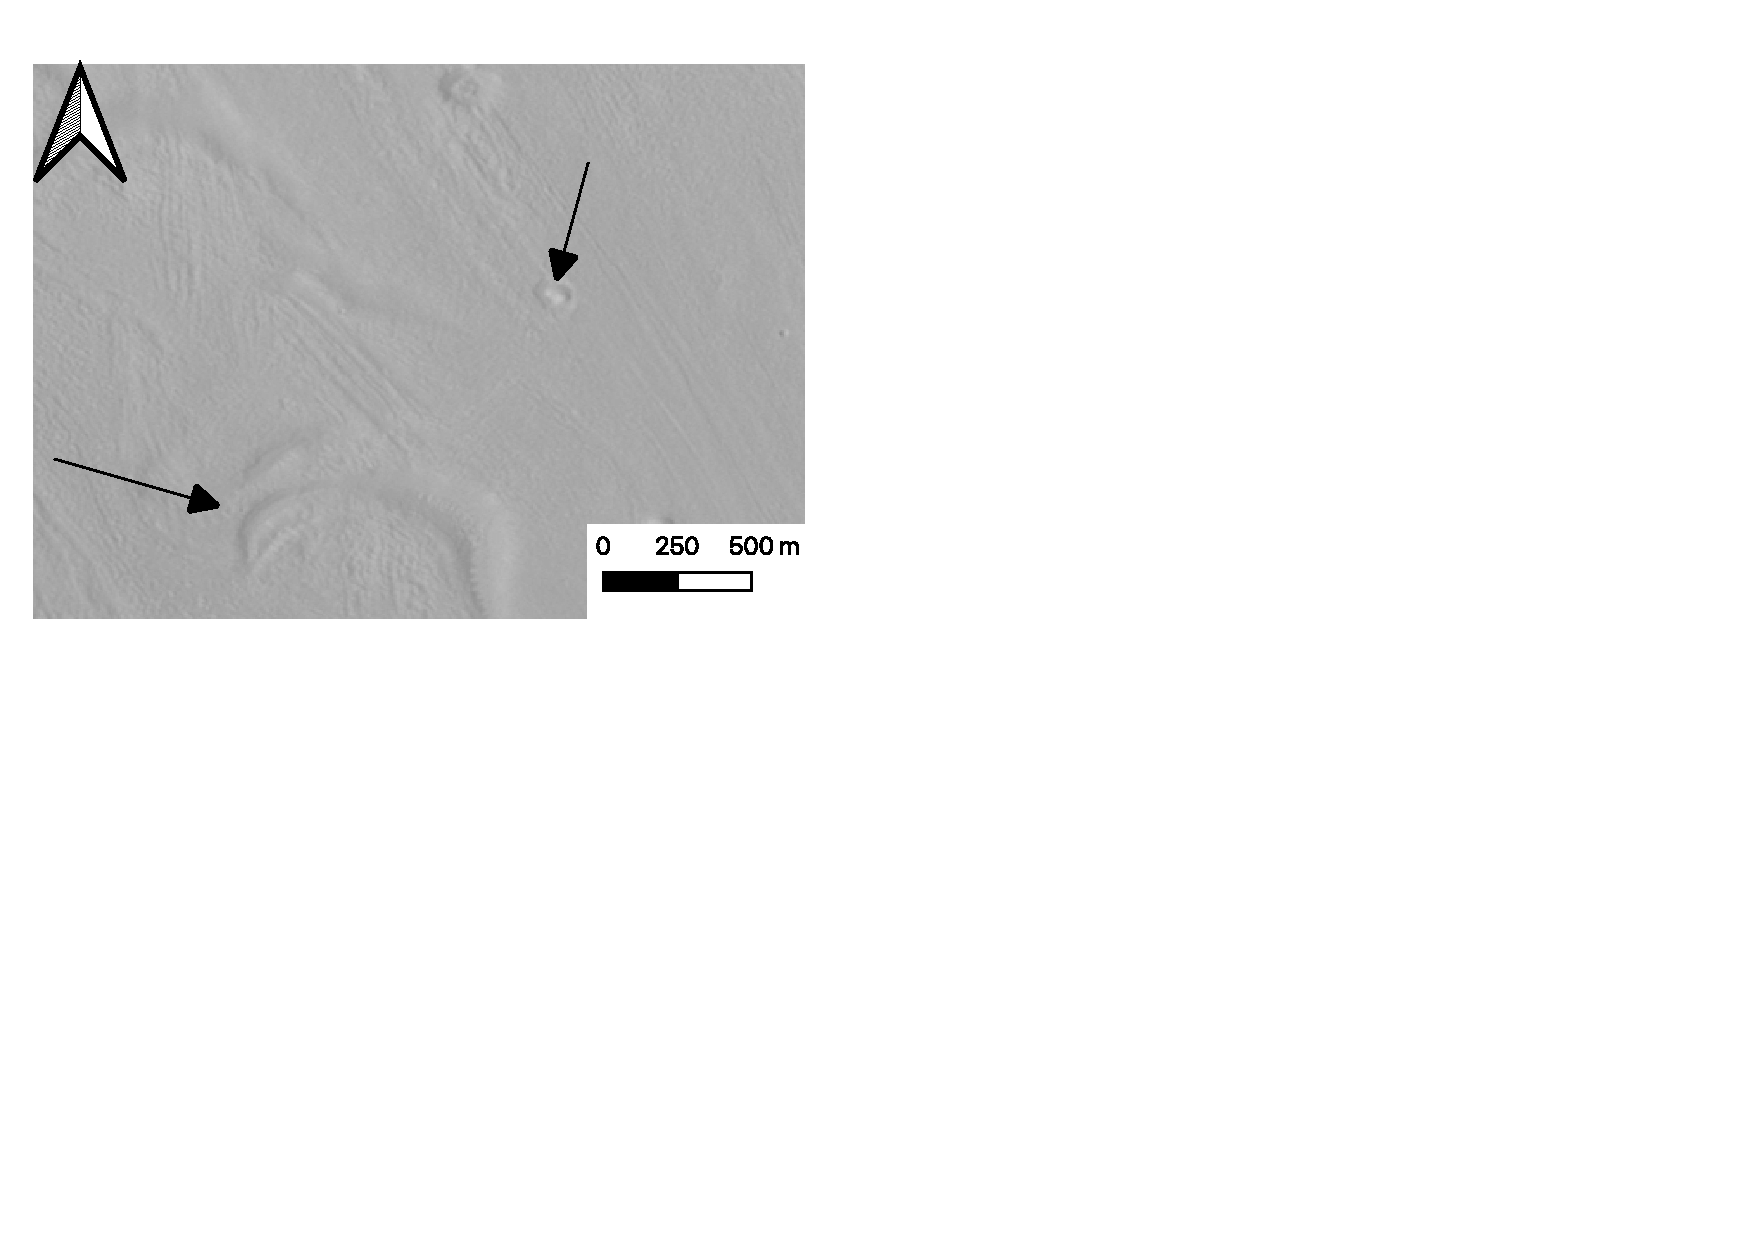
\includegraphics[
        width=\linewidth,
        height=0.65\textheight,
        keepaspectratio
    ]{Figures/CTX/IceActivityZoom_Img.pdf}
    \label{fig:IceActivityZoom_a}
\end{subfigure}
\hfill
\begin{subfigure}{0.48\textwidth}
    \centering
    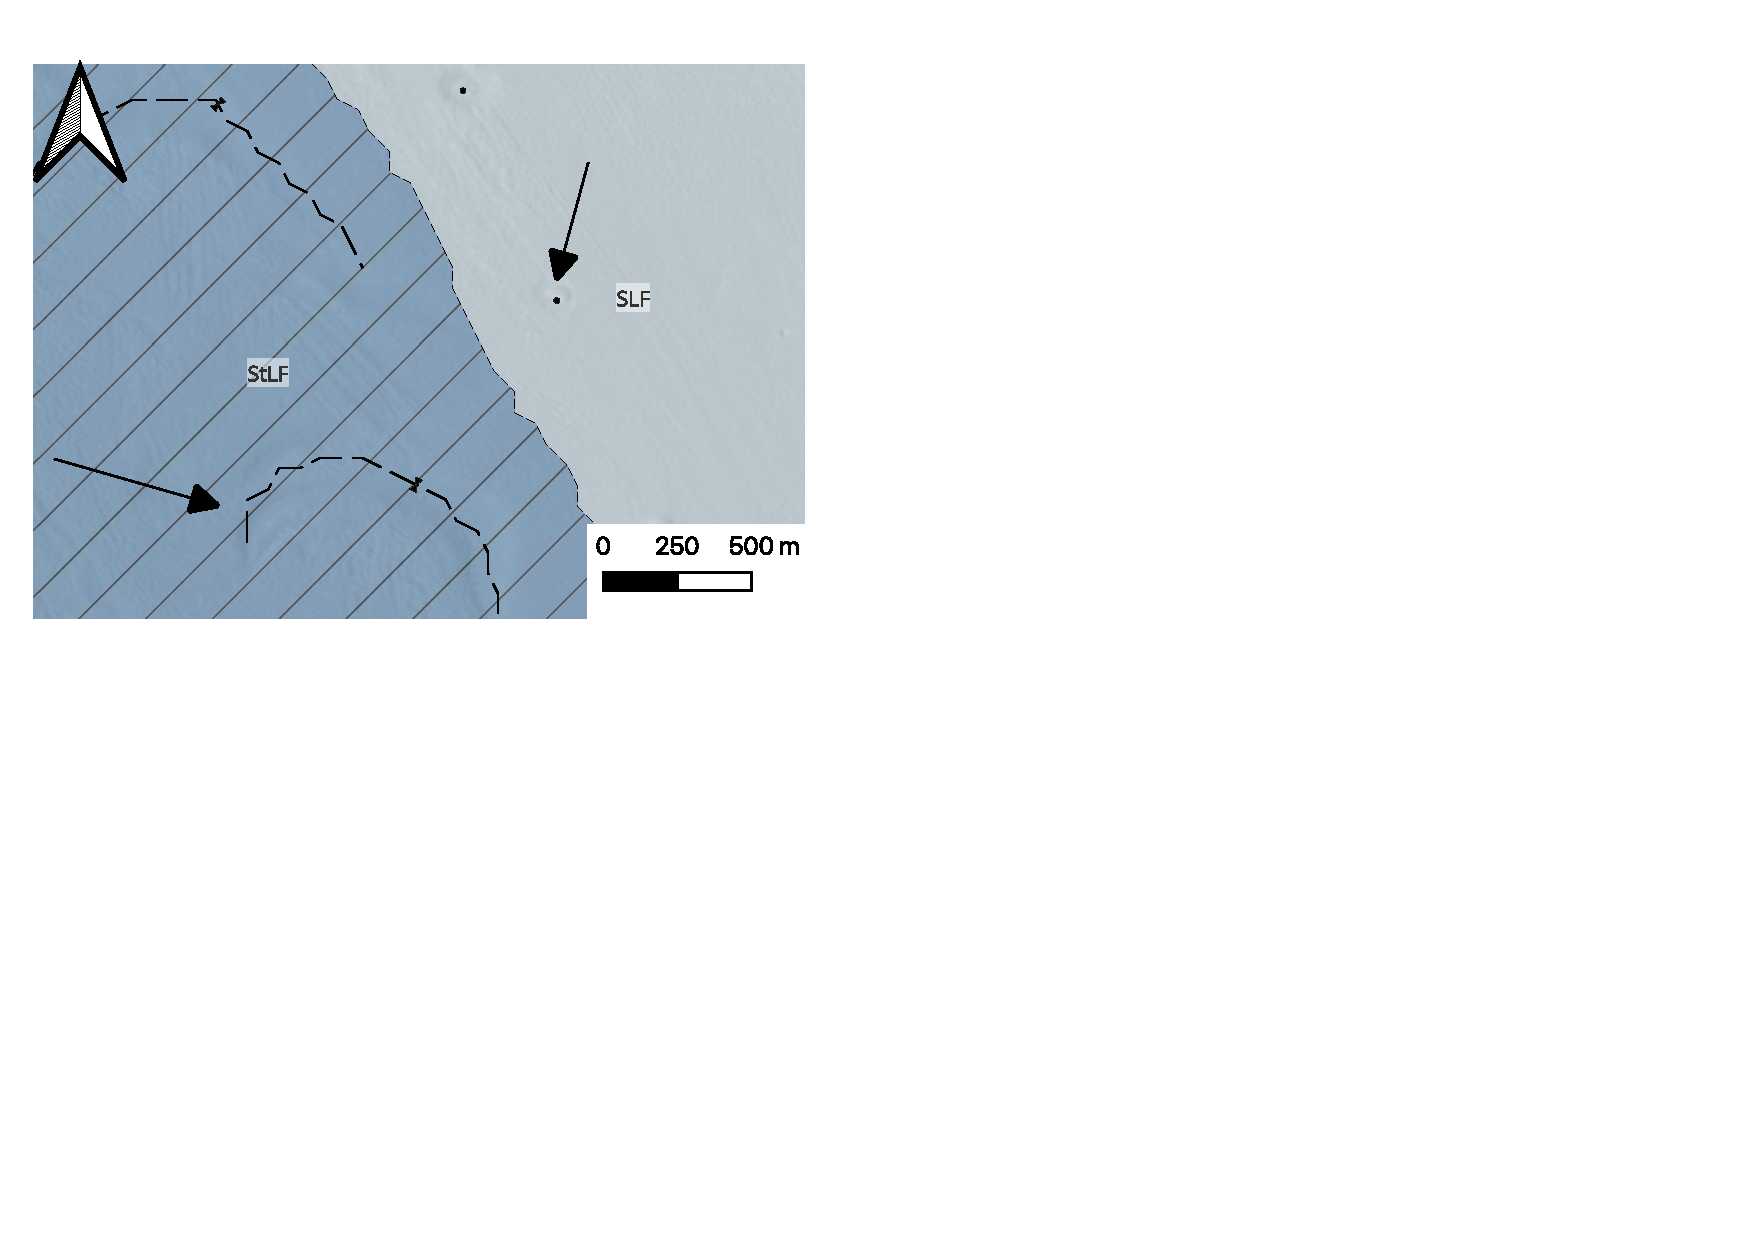
\includegraphics[
        width=\linewidth,
        height=0.65\textheight,
        keepaspectratio
    ]{Figures/CTX/IceActivityZoom_Map.pdf}
    \label{fig:IceActivityZoom_b}
\end{subfigure}

\caption{Sublimation-related erosional features near Mamers Valles. A ring-mold crater (right) and crevasse (left) are highlighted (centred at $34.61601^{\circ}$N, $16.97785^{\circ}$E).}
\label{fig:IceActivityZoom}

\end{figure}

\end{frame}

\againframe{RingMold}
